\documentclass[fleqn,10pt]{wlscirep}
\usepackage[utf8]{inputenc}
\usepackage[T1]{fontenc}
\usepackage{lineno}
\graphicspath{{./img/}{./pictures/}{./images/}}
\linenumbers

\usepackage[dvipsnames]{xcolor} % colors
\newcommand{\tom}[1]{{\textcolor{RedOrange}{#1}}}
\newcommand{\hh}[1]{{\textcolor{Green}{#1}}}
\usepackage{framed}

\newcommand{\ifinstruction}{1} % 1 for instruction, 0 for no instruction

%in the preamble
%--------------------------------
\usepackage{natbib}
\bibliographystyle{jabbr}
%--------------------------------

\title{$title$}

$for(by-author)$
\author[$for(it.affiliations)$$it.id$$sep$,$endfor$$if(it.corresponding)$,*$endif$]{$it.name.literal$}
$endfor$

$for(affiliations)$
\affil[$it.id$]{$it.name$, $it.department$, $it.city$, $it.state.literal$}
$endfor$

$for(by-author)$
\affil[*]{corresponding author(s): $it.name.literal$ ($it.email$) \tom{it.corresponding returns nothing} }
$endfor$

\begin{abstract}
$abstract$
\end{abstract}
\begin{document}

\flushbottom
\maketitle
%  Click the title above to edit the author information and abstract

\thispagestyle{empty}

$body$

\bibliography{references}

\noindent LaTeX formats citations and references automatically using the bibliography records in your .bib file, which you can edit via the project menu. Use the cite command for an inline citation, e.g. \cite{Kaufman2020, Figueredo:2009dg, Babichev2002, behringer2014manipulating}. For data citations of datasets uploaded to e.g. \emph{figshare}, please use the \verb|howpublished| option in the bib entry to specify the platform and the link, as in the \verb|Hao:gidmaps:2014| example in the sample bibliography file. For journal articles, DOIs should be included for works in press that do not yet have volume or page numbers. For other journal articles, DOIs should be included uniformly for all articles or not at all. We recommend that you encode all DOIs in your bibtex database as full URLs, e.g. https://doi.org/10.1007/s12110-009-9068-2.

\section*{Acknowledgements} 
$acknowledgements$

\section*{Author contributions statement}

$contributions$
Must include all authors, identified by initials, for example:
A.A. conceived the experiment(s), A.A. and B.A. conducted the experiment(s), C.A. and D.A. analysed the results. All authors reviewed the manuscript. 

\section*{Competing interests} (mandatory statement)

$competing$

% XXX Delete the section below later
\ifnum \ifinstruction=1
\section*{Figures \& Tables}


Figures, tables, and their legends, should be included at the end of the document. Figures and tables can be referenced in \LaTeX{} using the ref command, e.g. Figure \ref{fig:stream} and Table \ref{tab:example}. 

Authors are encouraged to provide one or more tables that provide basic information on the main ‘inputs’ to the study (e.g. samples, participants, or information sources) and the main data outputs of the study. Tables in the manuscript should generally not be used to present primary data (i.e. measurements). Tables containing primary data should be submitted to an appropriate data repository.

Tables may be provided within the \LaTeX{} document or as separate files (tab-delimited text or Excel files). Legends, where needed, should be included here. Generally, a Data Descriptor should have fewer than ten Tables, but more may be allowed when needed. Tables may be of any size, but only Tables which fit onto a single printed page will be included in the PDF version of the article (up to a maximum of three). 

Due to typesetting constraints, tables that do not fit onto a single A4 page cannot be included in the PDF version of the article and will be made available in the online version only. Any such tables must be labelled in the text as ‘Online-only’ tables and numbered separately from the main table list e.g. ‘Table 1, Table 2, Online-only Table 1’ etc.

\begin{figure}[ht]
\centering
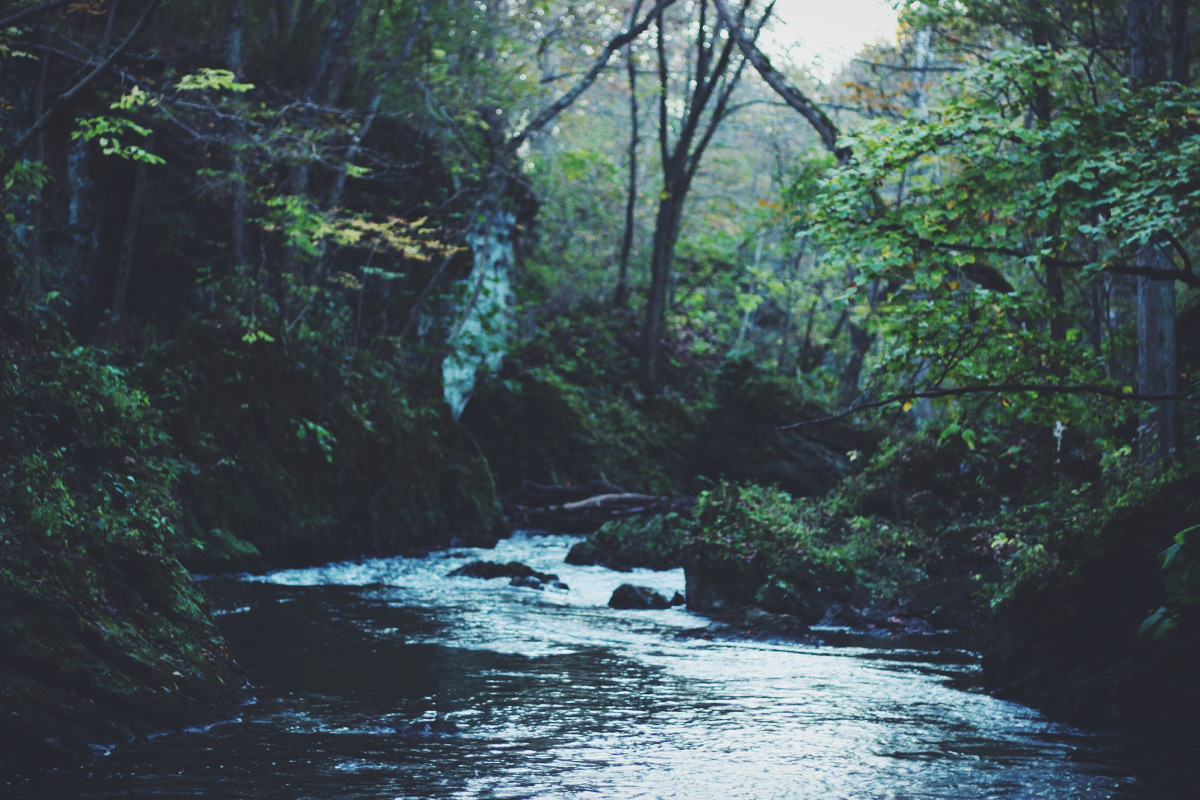
\includegraphics[width=\linewidth]{stream}
\caption{Legend (350 words max). Example legend text.}
\label{fig:stream}
\end{figure}

\begin{table}[ht]
\centering
\begin{tabular}{|l|l|l|}
\hline
Condition & n & p \\
\hline
A & 5 & 0.1 \\
\hline
B & 10 & 0.01 \\
\hline
\end{tabular}
\caption{\label{tab:example}Legend (350 words max). Example legend text.}
\end{table}
\fi

\end{document}